\section{Results} \label{sec:results}
In order to investigate how \xQ{} performs on a more realistic scenario the VIP escort problem introduced in Sec.~\ref{sec:vip_escort}. While the original escort problem is defined as a POMDP with, here we investigate a somewhat simpler version of the problem, and instead use fully observable MDPs. This is reasonable because \xQ{} operates on reward distributions, which are produced by policies on any decision making problem. The benefit of using MDPs is that they are computationally less burdensome than POMDPs, while still enabling complex decision making.

In order to find a policy for the MDP, a Monte-Carlo Tree Search (MCTS) solver will be used. As the name suggests MCTS involves building a tree from the starting state of the UGV and simulating a specified number of actions into the future and calculates the utility of each state. This process is repeated many times, and the utilities of each state are updated after each iteration of search. The actions selected by MCTS are based not only on the current utility of the state, but an exploration parameter that helps ensure that the search doesn't simply exploit the greatest known utilities. An MCTS solver is convenient to use during these experiments because the quality of the solver can be changed by modifying the parameters.

\begin{figure}[tbp]
    \centering
    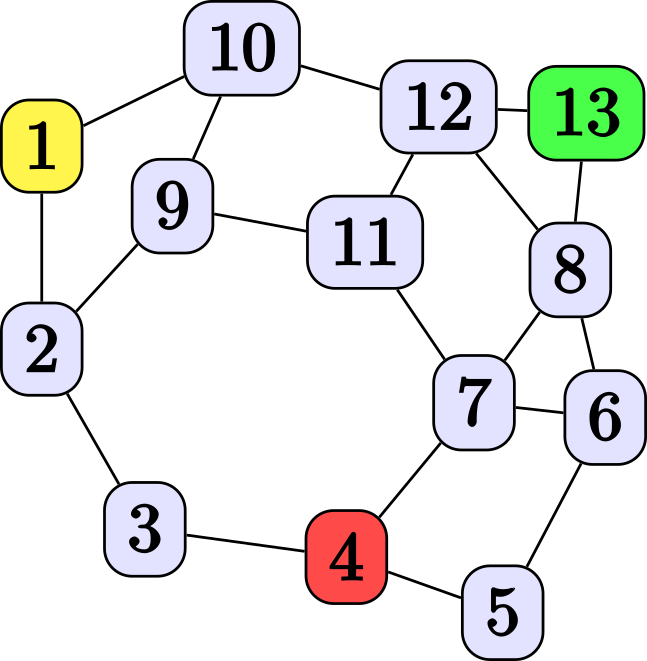
\includegraphics[width=0.4\linewidth]{Figures/original_roadnet.png}
    \caption{Diagram of the `Road Network' layout. Node 1 (yellow) is the start location of the UGV. Node 4 (red) is the start location of the pursuer vehicle. Node 13 (green) is the exit node.}
    \label{fig:roadnet}
\end{figure}

The road network is represented as shown in Fig.~\ref{fig:roadnet}. The UGV begins at the yellow node (node 1), the pursuer begins at the red node (node 4), and the desired exit is indicated by the green node (node 13). The problem is defined by the following parameters:

\tymin=80pt
\begin{table}[]
\footnotesize
\caption{Table of parameters for the simplified VIP escort problem}
\begin{tabulary}{\linewidth}{CL}
\hline
Parameter    & Description\\
\hline
p_{trans}    & The transition probability of the UGV. This is the probability that the UGV will move in the desired direction when attempting to move. There is a probability of $1-t_prob$ that it will go to a different neighboring cell. \\
d            & MDP discount factor\\
N            & The number of nodes included in the road\\
% Mean Degree  & The target mean degree to which random networks are generated\\
e_{mcts}     & The exploration constant parameter of the MCTS.\\
d_{mcts}     & The depth of the MCTS tree\\
its_{mcts}   & The number of Monte-Carlo simulations to run to find the policy\\
rwd_{exit}   & The reward for the UGV successfully exiting the road network\\
rwd_{caught} & The reward for the UGV being caught by the pursuer\\
rwd_{sense}  & The reward for making a movement\\
\hline
\end{tabulary}
\end{table}
\begin{table*}
    \footnotesize
    \centering
    \caption{Parameters used for the different experiments}
    \label{tab:exps}
    \begin{tabular}{llcccccccccc} \toprule
        &\multicolumn{10}{c}{Parameters} \\ \cmidrule(r){3-12}
        \#  & Variable(s) & Network &p_{trans}&d&N&e_{mcts}&d_{mcts}&its_{mcts}&rwd_{exit}&rwd_{caught}&rwd_{sense} \\ \midrule
        1 & \{d_{mcts}\} & Fig.~\ref{fig:roadnet} & $[0.0,1.0]$ & $0.95$ & 13 & $[1000.0]$ & [1:1:10] & 100 & 2000 & -2000 & -100\\
        2 & \{d_{mcts}\} & Fig.~\ref{fig:med_roadnet} & $[0.0,1.0]$ & $0.95$ & 45 & $[2000.0]$ & [1:3:28] & 1000 & 2000 & -2000 & -100\\
        3 & \{p_{trans}\}& Fig.~\ref{fig:roadnet} & $[0.0,1.0]$ & $0.95$ & 13 & $[1000.0]$ & [8,3,1] & 1000 & 2000 & -2000 & -100\\
        4 & \{p_{trans},e_{mcts}\} & Fig.~\ref{fig:roadnet} & $[0.0,1.0]$ & $0.95$ & 13 & $[10.0,1000.0]$ & [8,3,1] & 1000 & 2000 & -2000 & -100\\
    \end{tabular}
\end{table*}

Three evaluations were completed. First, \xQ{} was calculated for MCTS solvers with different parameters. (all other parameters were held constant). Second, \xQ{} was evaluated for a candidate solver with varying task parameters. Finally, \xQ{} was evaluated for a candidate solver with different task \emph{and} solver parameters.

\subsection{Varying A Solver Parameter}
This evaluation involved experiments 1 and 2 from Table~\ref{tab:exps}. The MCTS solver was run on each of the two networks ($N=13$ for 1, and $N=45$ for 2) with different depths. In each case one of the solvers was chosen as the trusted one (i.e. chose a `good' solver, but not necessarily the `best' one). In the case of experiment 1 \solvestar{} was the $d_{mcts}=9$ solver, and in experiment 2 \solvestar{} was the $d_{mcts}=25$ solver. A surrogate \surrogate{} was not used for this evaluation, instead \rwdstar{} was calculated directly and used for comparison.

The results for experiment 1 are shown in Fig.~\ref{fig:mcts_d}. As expected \xQ{} between the trusted solver and itself is 1.0. We see that candidate solvers depth 6 through 10 are about equivalent to the trusted solver (and each other), which indicates they are similarly capable of solving the problem. Whereas candidate solvers with depth 1 through 3 are much less capable than the trusted solver.

The results of experiment 2 are shown in Fig.~\ref{fig:mcts_d_med}, where the trusted solver with $d_{mcts}=5$ has been selected. According to the plot only solvers of depth 22, and 28 have similar capability to the trusted solver. Note, that the $d_{mcts}=1$ solver has $x_Q=0.83$, this is most possibly due to the fact that the depth 1 solver will make decisions based on little foresight, while solver with depths from 4 to 19 have enough foresight to hesitate and accumulate negative rewards from not moving quickly.

An important insight is that while the $d_{mcts}=9$ solver is very capable of solving the small network from Fig.~\ref{fig:roadnet}, that performance does not extent to the medium sized network from Fig.~\ref{fig:med_roadnet}. The $d_{mcts}=7 \text{ and} 10$ solvers are very incapable compared to the trusted solver of $d_{mcts}=25$, this is reflected by the value of \xQ.

\begin{figure}[tbp]
    \centering
    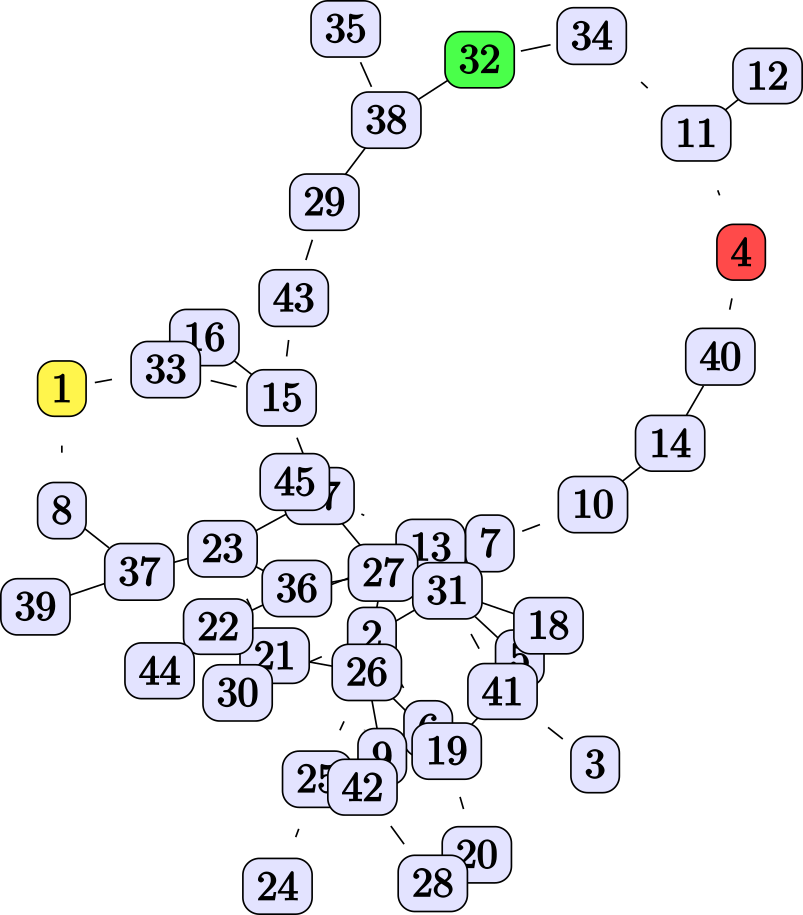
\includegraphics[width=0.4\linewidth]{Figures/medium_roadnet.png}
    \caption{Diagram of a randomly generated road network with that is quite a bit larger ($N=45$) than the original shown in Figure \ref{fig:roadnet}.}
    \label{fig:med_roadnet}
\end{figure}

\begin{figure}[tbp]
    \centering
    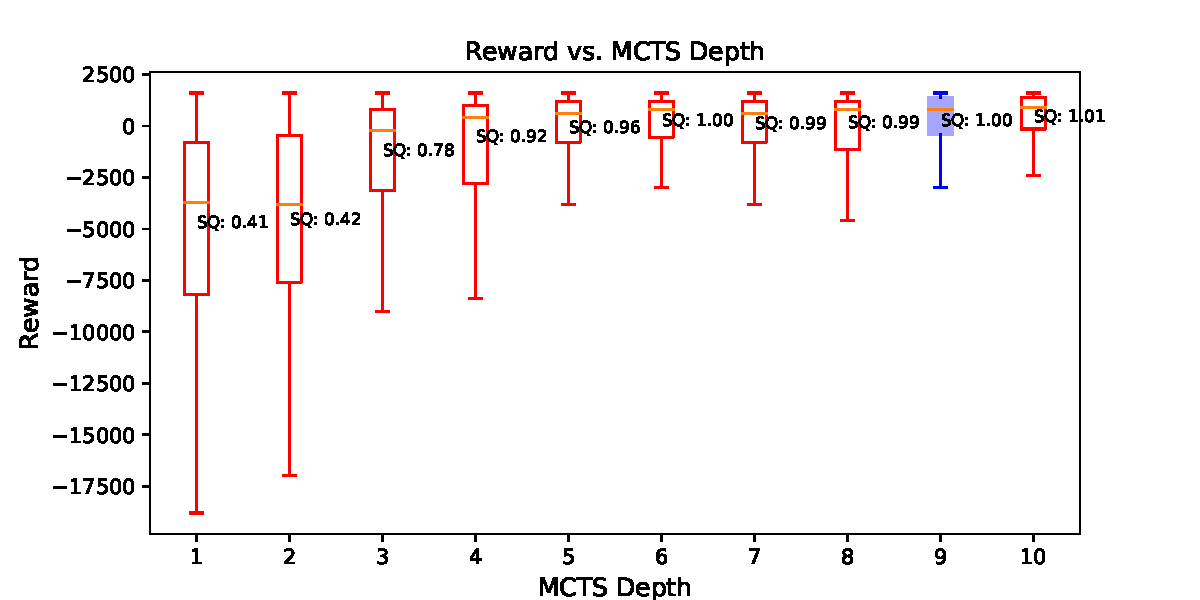
\includegraphics[width=1.0\linewidth]{Figures/sq_roadnet_mcts_i100e1000.pdf}
    \caption{Results from Experiment 1. Varying the $d_{mcts}$ parameter for the road network in Figure \ref{fig:roadnet}. The \xQ{} values being calculated are with respect to the trusted distribution highlighted, depth equal 9.}
    \label{fig:mcts_d}
\end{figure}
\begin{figure}[tbp]
    \centering
    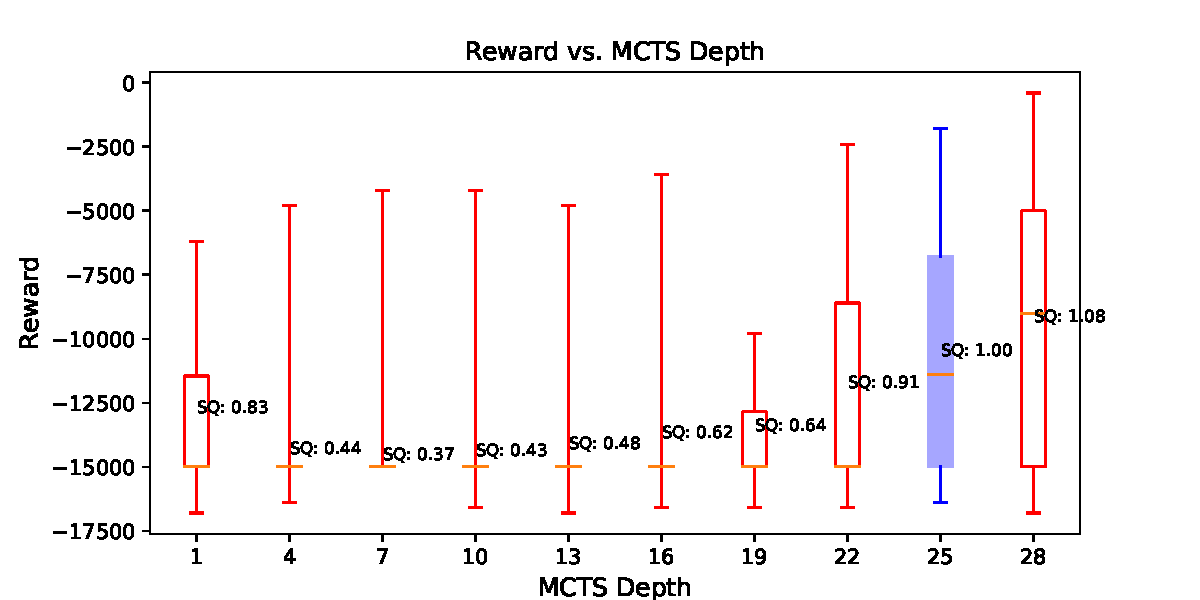
\includegraphics[width=1.0\linewidth]{Figures/sq_mednet_mcts_i1000e2000.pdf}
    \caption{Results form Experiment 2. Varying the $d_{mcts}$ parameter for the road network in Figure \ref{fig:med_roadnet}. The \xQ{} value being calculated are with respect to the trusted solver of depth 25.}
    \label{fig:mcts_d_med}
\end{figure}

\subsection{Varying A Task Parameter}
Experiment 3 was used for this evaluation, \solverstar{} is a depth 8 solver, while the two candidate solvers were depth 3 and depth 1. The surrogate model \surrogate{} was learned using a two generic deep neural networks  with three hidden layers. One network to learn to predict the mean reward, and the other to predict the standard deviation (\surrogate{} here is a combination two models). In a fairly simple problem such as this one a DNN of this configuration is likely overkill, but it demonstrates the possibility of using an arbitrarily complex black box model for \surrogate.

Figure~\ref{fig:tprob_ok} shows the results for the candidate solver with $d_{mcts}=3$ at two different values of $p_{trans}$. At $p_{trans}=0.25$ the candidate solver is slightly more capable than the trusted solver. Whereas, at $p_{trans}=0.75$ the candidate solver is slightly less capable.

Figure~\ref{fig:tprob_bad} shows the results for the candidate solver with $d_{mcts}=1$ at two different values of $p_{trans}$. At $p_{trans}=0.25$ the candidate solver is moderately less capable than the trusted solver. Whereas, at $p_{trans}=0.75$ the candidate solver is slightly much less capable.

\begin{figure}[tbp]
    \centering
    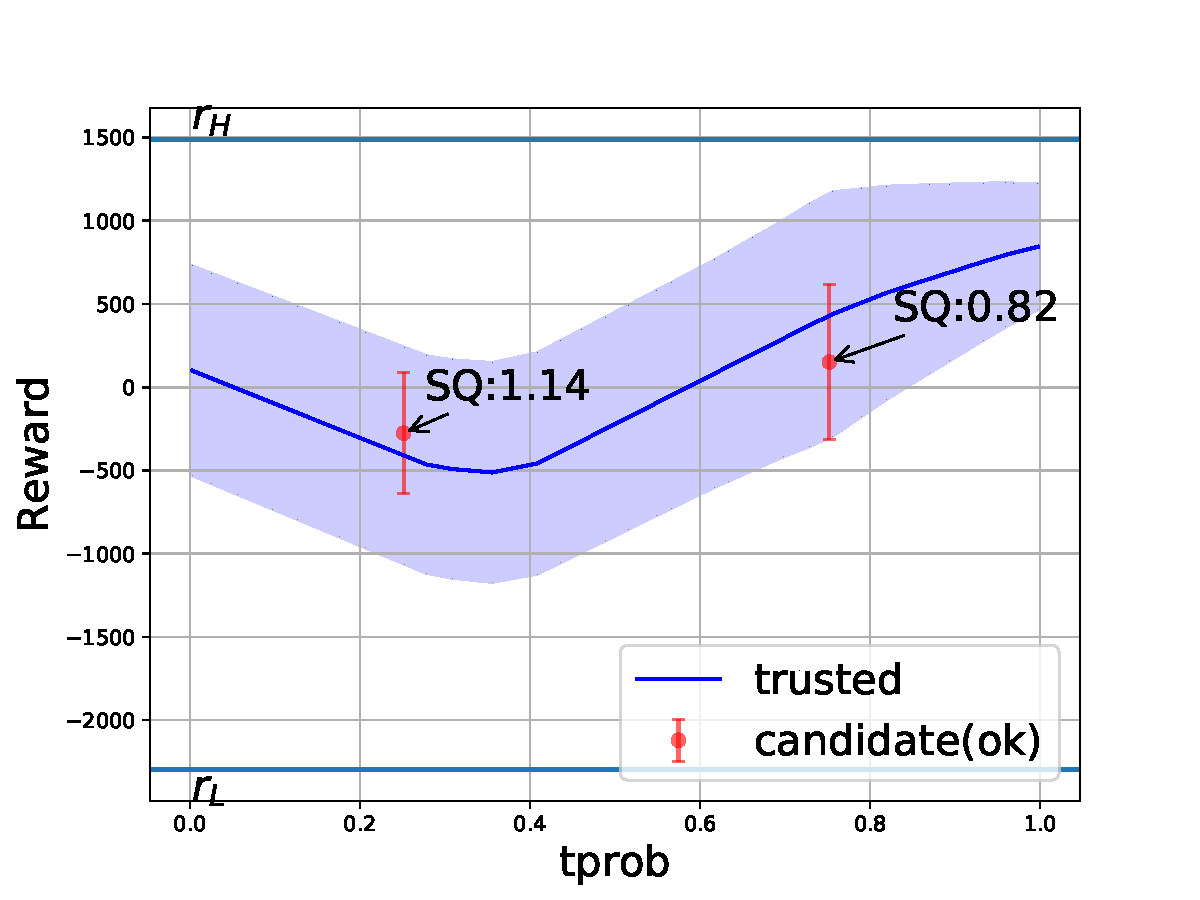
\includegraphics[width=0.9\linewidth]{Figures/transition_vary_tprob_ok.pdf}
    \caption{Comparison of candidate solver of depth 3 to that of a trusted solver with depth 8. Two separate values for \xQ{} (displayed as SQ), and $p_{trans}$ (tprob) are displayed.}
    \label{fig:tprob_ok}
\end{figure}
\begin{figure}[tbp]
    \centering
    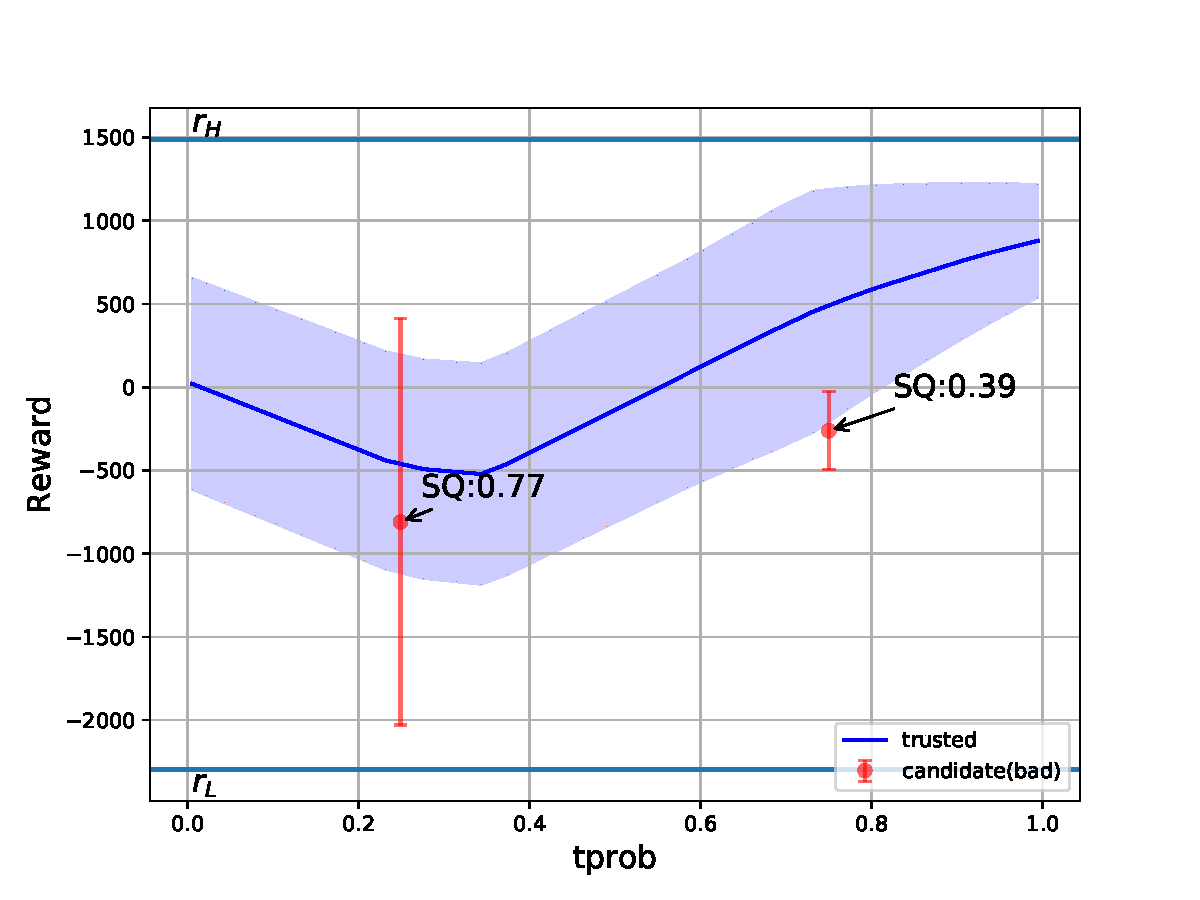
\includegraphics[width=0.9\linewidth]{Figures/transition_vary_tprob_bad.pdf}
    \caption{Same as Fig.~\ref{fig:tprob_ok} for candidate solver of depth 1.}
    \label{fig:tprob_bad}
\end{figure}

\subsection{Varying Task and Solver Parameters}
Experiment 4 was used for this evaluation, \solverstar{} is a depth 8 solver, while the two candidate solvers were depth 3 and depth 1. Both $p_{trans}$ and $e_{mcts}$ were variable for the experiments. The results are found in Figs.~\ref{fig:tprob_emcts_ok} and \ref{fig:tprob_emcts_bad}. The surrogate \surrogate{} used here is the same as in the previous evaluation (i.e. two DNNs to predict mean and standard deviation).

Figure~\ref{fig:tprob_emcts_ok} shows the results for the candidate solver with $d_{mcts}=3$ at two different values of $p_{trans}$. At $p_{trans}=0.25$ the candidate solver is slightly more capable than the trusted solver. Whereas, at $p_{trans}=0.75$ the candidate solver is slightly less capable.

Figure~\ref{fig:tprob_emcts_bad} shows the results for the candidate solver with $d_{mcts}=1$ at two different values of $p_{trans}$. At $p_{trans}=0.25$ the candidate solver is moderately less capable than the trusted solver. Whereas, at $p_{trans}=0.75$ the candidate solver is slightly much less capable.

\begin{figure}[tbp]
    \centering
    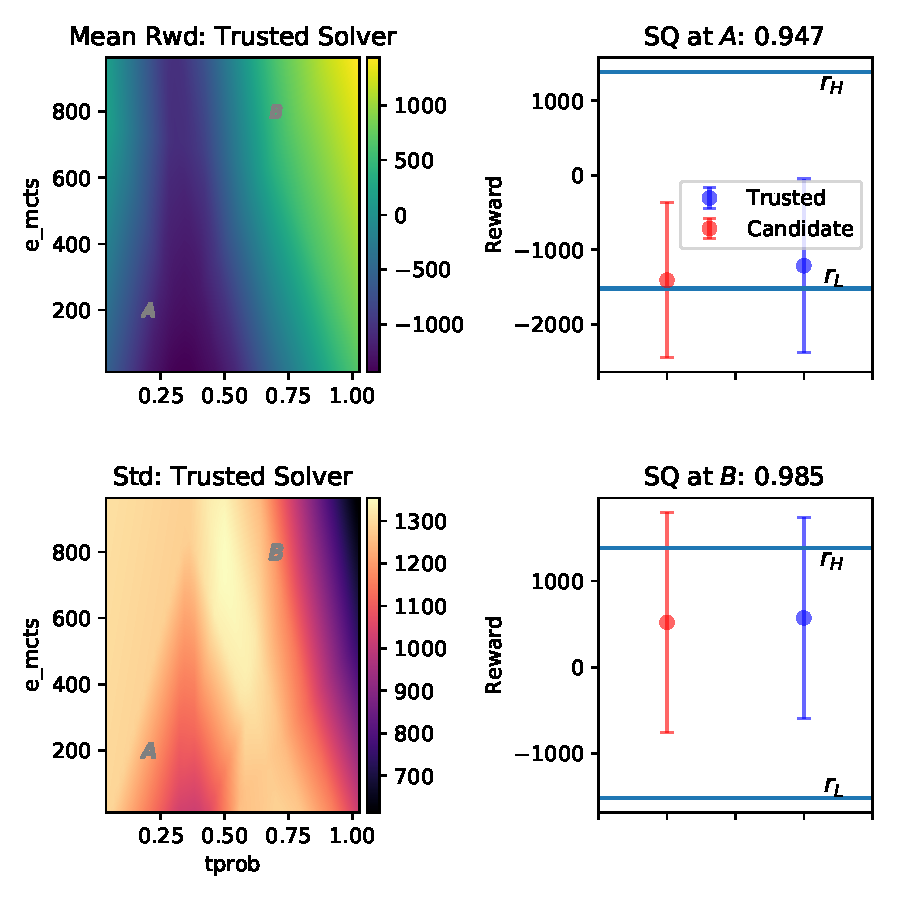
\includegraphics[width=0.9\linewidth]{Figures/transition_e_vary_e_mctstprob_ok.pdf}
    \caption{Comparison of candidate solver of depth 3 to that of a trusted solver with depth 8. The top-left figure shows the mean reward of the trusted solver, the bottom-left is the standard deviation of the trusted solver. The top-right figure shows the value of \xQ{} (SQ) at point A. The two blue lines indicate $r_H$ and $r_L$. The bottom-right figure shows \xQ{} at point B.}
    \label{fig:tprob_emcts_ok}
\end{figure}
\begin{figure}[tbp]
    \centering
    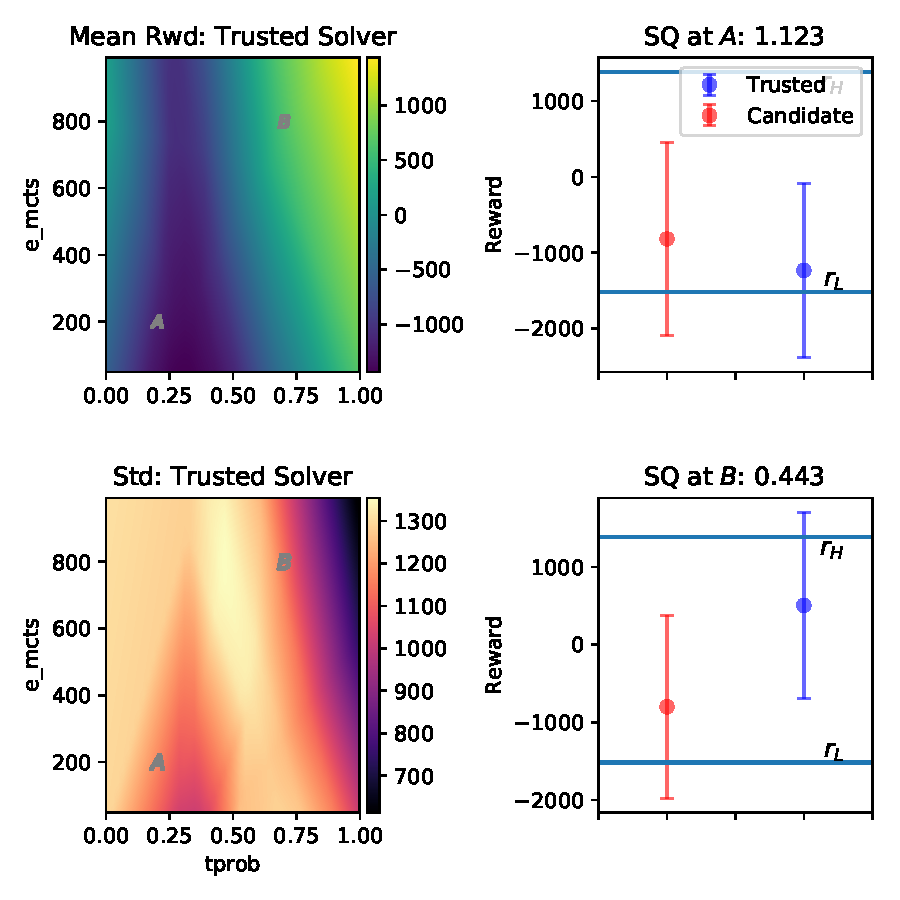
\includegraphics[width=0.9\linewidth]{Figures/transition_e_vary_e_mctstprob_bad.pdf}
    \caption{Same as Fig.~\ref{fig:tprob_emcts_ok} for candidate solver of depth 1.}
    \label{fig:tprob_emcts_bad}
\end{figure}
